\section{Implementation of Hartree-Fock}
\label{sec:ImplHF}
Our code contains an own class, called \textit{HartreeFock}, which allows the user to prepend a \mbox{Hartree-Fock} (HF) to the SRG calculation. The purpose is to transform an ordinary harmonic oscillator to a Hartree-Fock basis, which can be used as input for the following computations. To gain as much efficiency as possible, we structured the code to be in line with the data structures of the in-medium SRG case, such that a direct use of the transformed elements is possible. However, the class can without any problems be used for the calculations preceding free-space SRG, too.\\
In practice, the class receives the untransformed one- and two-body elements $\langle \alpha |\hat{h}^{(0)}| \gamma\rangle$ and $\langle \alpha \beta ||\gamma\delta\rangle$ of the Hamiltonian and transforms them using a coefficient matrix. In our case, the one-body elements are given by the single-particle energies and the tp-elements are obtained using the code of Simen Kvaal \cite{Kvaalcode}.\\
The transformation occurs in two steps: First, we perform a HF calculation based on the convergence of the HF energy. This yields the coefficient matrix $C$, which is used to transform the basis elements. \\
In the following, we will explain both steps in detail and present the most important aspects of our implementation.

\subsection{Hartree-Fock calculation}
Our Hartree-Fock calculation is based on the explanations of section \ref{sec:HF}, in particular on \mbox{Eqs. (\ref{eq:HF2}), (\ref{eq:HF3})} and (\ref{eq:HF4}). The main algorithm is implemented in one routine, which takes as input an untransformed single-particle basis and returns the HF energy, as well as the $C$-matrix which can be used for a subsequent basis transformation.
As explained in section \ref{sec:HF}, the
he HF orbitals are linear combinations of single-particle functions
\[ 
|p\rangle = \sum_{\alpha} C_{p\alpha} |\alpha\rangle.
\]
where $|\alpha\rangle$ is the set of orthonormal single-particle functions that spans the chosen model space. In our case, this is given by a harmonic oscillator basis. The idea is to vary the coefficients in this expansion, such that the HF energy, given in Eq.~(\ref{eq:HF1}), is minimized.  For this purpose, the HF equations (\ref{eq:HF4}) are solved iteratively. The complete algorithm is summarized in figure \ref{fig:HFbox}. In the following, we will look at the details of the algorithm and demonstrate how we implemented the different stages in our class \textit{HartreeFock}.

\begin{figure}
\begin{framed}
\begin{center}
\textbf{Hartree-Fock algorithm}
\end{center}
\textbf{Input}: Untransformed basis elements $\langle \alpha |\hat{h}^{(0)}| \gamma\rangle$ and $\langle \alpha \beta ||\gamma\delta\rangle$.

\begin{enumerate}
\item Initialize the coefficient matrix to $C=\hat{1}$.
\item While not converged:
\begin{enumerate}
\item Use $C$ to compute $\hat{h}^{HF}$ according to Eq.~(\ref{eq:HF3}).
\item Diagonalize $\hat{h}^{HF}$ to obtain its eigenvectors.
\item Let those eigenvalues define the coefficient vectors for the next guess of $C$.
\item Compute the new HF energy $E \left[ \Phi_0^{HF}\right]$ according to Eq.~(\ref{eq:HF2}).
\item Determine the difference between $E \left[ \Phi_0^{HF}\right]$ of current and previous iteration.
\end{enumerate}
\end{enumerate}
\textbf{Output}: HF energy $E \left[ \Phi_0^{HF}\right]$ and coefficient matrix $C$.
\end{framed}
\caption{Summary of the Hartree-Fock algorithm.}
\label{fig:HFbox}
\end{figure}

The first step is to initialize the coefficient matrix $C$. For a pure HF calculation, where one is only interested in the HF energy, the dimension of this matrix is only required to be $N\times n_{sp}$, where $N$ and $n_{sp}$ denote the number of particles and single-particle states, respectively. The orbital of electron $k$ is then associated with the $k$th column of the matrix and this vector,
\[
C_k = \left(\begin{array}{c}
C_{1k}\\
C_{2k}\\
\dots\\
C_{nk}
\end{array}\right),
\]
is used for the HF equation (\ref{eq:HF4}).
However, since for a basis transformation all eigenvectors of the HF-matrix are needed, our $C$-matrix has dimension $n_{sp}\times n_{sp}$. At the beginning of the calculation, the coefficient matrix is initialized to $C=\hat{1}$, which is equivalent to starting with an untransformed basis.\\
For each HF iteration, we then proceed as follows:
First, we use the $C$-matrix to compute the HF-matrix $\hat{h}^{HF}$ according to Eq.~(\ref{eq:HF3}). The challenge hereby is to store $\hat{h}^{HF}$ in a way that minimizes required space in memory and allows an efficient diagonalization. Inspired by the procedure of \cite{Marte,Christoffer}, we store $\hat{h}^{HF}$ in block-form:
Similar to storing the Hamiltonian in our SRG part, we use that $M$ and $M_s$ are conserved, suggesting that $\hat{h}^{HF}$ is block-diagonal in $M$ and $M_s$. Therefore we store the HF-matrix as an array of those blocks, which allows to perform blockwise diagonalization later on. For setting up the blocks, we proceeded similar as \cite{Marte}, although we adjusted the implementation to our code structure and optimized it. We have adopted the  computational trick presented there, namely introducing another matrix, called \textit{rho}, to speed up convergence. For details, we refer to \cite{Marte}.\\
Having computed all blocks of $\hat{h}^{HF}$ using the $C$-matrix, the next step is to diagonalize those blocks. In our code, we employ the function \textit{eig\_sym} of the Armadillo library, which refers to LAPACK functions for diagonalizing.\\
As summarized in the algorithm in figure \ref{fig:HFbox}, we let 
those eigenvalues define the coefficient vectors for the next guess of $C$.  The next step is to
compute the new HF energy $E \left[ \Phi_0^{HF}\right]$. Since the non-interacting part $\hat{h}_0$ of our Hamiltonian is diagonal, Eq.~(\ref{eq:HF2}) can be simplified to
\be
E \left[ \Phi_0^{HF}\right] = \sum_i \sum_{\alpha} C_{i\alpha}^2 \epsilon_{\alpha}  + \frac{1}{2} \sum_{ij} \sum_{\alpha\beta\gamma\delta} C_{i\alpha}^* C_{j\beta}^* C_{i\gamma} C_{j\delta} \langle \alpha\beta || \gamma\delta\rangle,
\label{eq:HF2mod}
\ee
where $\epsilon_{\alpha} = \langle \alpha |\hat{h}_0 |\alpha\rangle$ are the single-particle energies. Each iteration, the new HF energy is compared with the one of the previous iteration and if the energy has not changed within a certain tolerance interval, it is said to have converged and we end the iterations. The final result of all iterations are the HF energy $E \left[ \Phi_0^{HF}\right]$ and the coefficient matrix $C$.

\paragraph{Improving efficiency}
To make the Hartree-Fock implementation as effective a possible, we took two major steps: \\
First, we try to rewrite as many sums as possible into matrix operations, similar to the optimizations of the SRG code. Inspired by the code of \cite{Christoffer}, we define a new matrix
\be 
C_{pq}^i = \sum_k C_{kp} C_{kq},
\label{eq:cinner0}
\ee
which can be expressed by a matrix-matrix multiplication the following way:
\[
C^i = C_{h\times all}^T \cdot C_{h\times all},
\]
where '$\cdot$' denotes matrix multiplication and $T$ the matrix transpose. The matrix $C_{h\times all}$ has dimension $N\times n_{sp}$ and contains the first $N$ columns of the $C$-matrix, where $N$ is the number of particles. With the matrix $C^i$, Eq.~(\ref{eq:HF2}) can be simplified to
\be 
E\left[\Phi_0^{HF}\right] = \sum_{\alpha\beta} C_{\alpha\beta}^i \langle \alpha | \hat{h}_0 | \beta \rangle + \frac{1}{2} \sum_{\alpha\beta\gamma\delta} C_{\alpha\gamma}^i C_{\beta\delta}^i \langle \alpha \beta || \gamma\delta\rangle.
\label{eq:cinner1}
\ee
That way, the first term is reduced from $\mathcal{O}(N n_{sp}^2)$ to $\mathcal{O}(n_{sp}^2)$ and the second one from $\mathcal{O}(N^2 n_{sp}^4)$ to $\mathcal{O}(n_{sp}^4)$, where  $n_{sp}$ denotes the number of single-particle states. This saves an enormous number of floating-point operations, especially for large numbers of particles and considered shells $R$. 

Additionally, we found another feature which allows considerable simplifications: Both matrices $C$ and $C^i$ are extremely sparse, i.e. most of their elements are zero, as illustrated in figure \ref{fig:sparsity}. When updating the HF energy according to Eq.~(\ref{eq:cinner1}), this means that most of the contributions are zero. 

\begin{figure}
\begin{center}
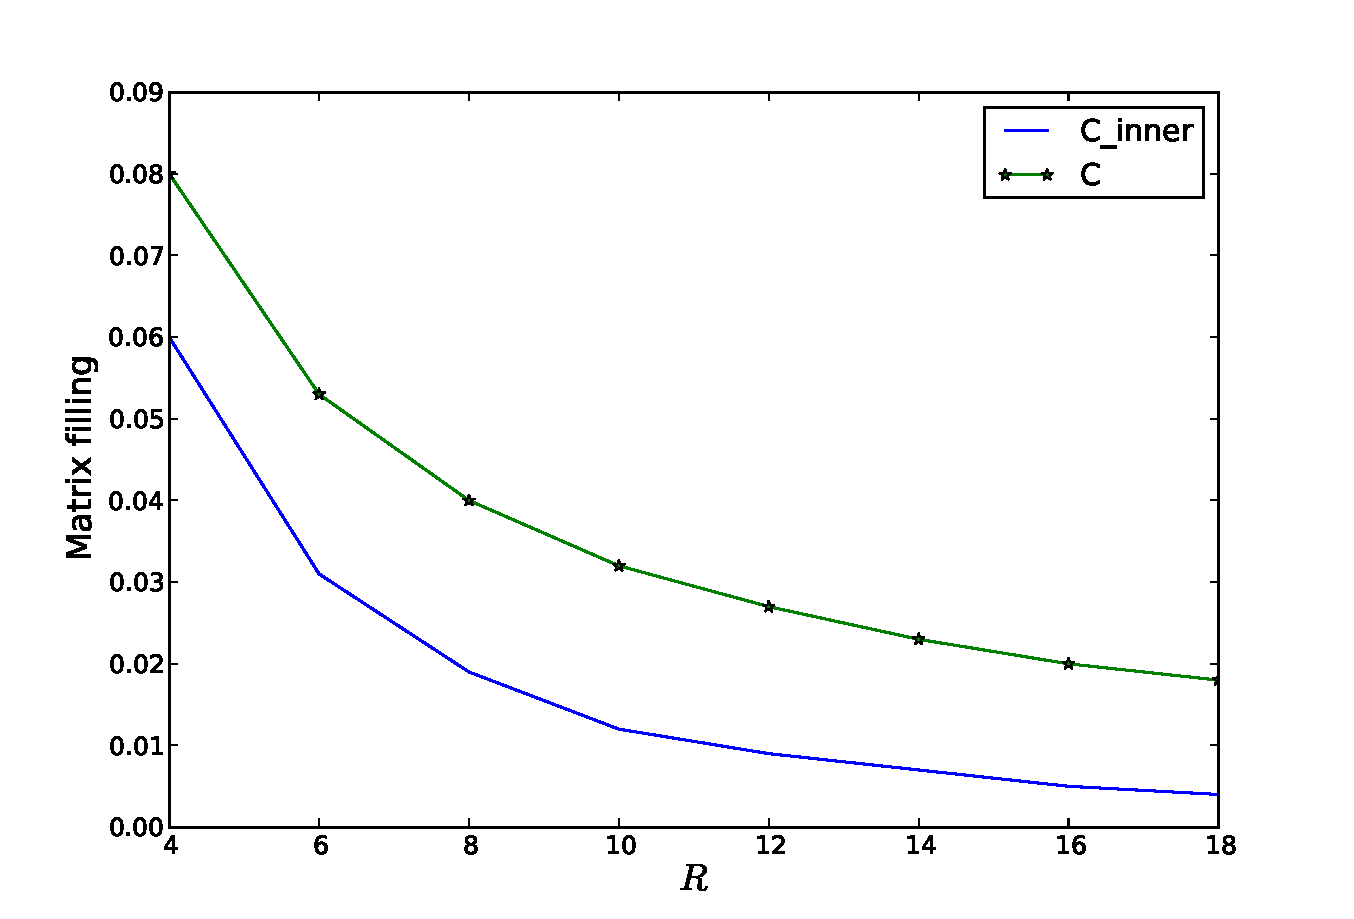
\includegraphics[scale=0.4]{../Plots/sparsity.pdf}
\caption{Sparsity of the coefficient matrices for systems with $N=2$ particles. The filling of the matrices is given by the percentage of non-zero elements.}
\label{fig:sparsity}
\end{center}
\end{figure}

We now tried to find a way to make use of this sparsity and avoid adding contributions that are known to be zero in advance. For this reason, we have introduced a new array, which saves for each index $i$ those indices $j$ that correspond to non-zero matrix elements $C_{ij}$. Instead of summing over all indices $\alpha,\beta,\gamma,\delta$, this allows for the second term of Eq.~(\ref{eq:cinner1}) to sum over only those combinations $\alpha,\gamma$ and $\beta,\delta$, such that the corresponding matrix elements $C_{\alpha\gamma}^i$ and  $C_{\beta\delta}^i$ are different from zero. The respective implementation can be found in listing \ref{lst:HF0}.

\begin{lstlisting}[float, caption={Calculation of the two-body contribution to the Hartree-Fock energy as given in Eq.~(\ref{eq:cinner1}). To minimize the number of terms, the array \textit{cCombs} contains those combinations of indices $p$ and $q$ such that the matrix elements $C_{pq}^i$ are different from zero. Parallelization is performed with OpenMP, where the clause \textit{reduction} ensures that all contributions are properly summed up.}, label={lst:HF0}]
#pragma omp parallel for private(alpha, gamma, beta, delta) reduction(+:hf_ret)
    for (alpha = 0; alpha < nsp; alpha++)
        for (int c = 0; c < cCombs[alpha].size(); c++) {
            gamma = cCombs[alpha][c];
            for (beta = 0; beta < nsp; beta++)
                for (int d = 0; d < cCombs[beta].size(); d++) {
                    delta = cCombs[beta][d];
                    hf_ret +=  C_inner(alpha, gamma) * C_inner(beta, delta)
                            * Sys->H->get_v_elem(alpha, beta, gamma, delta, Sys->H->mat_elems);
                }
        }
    
    hf_ret *= 0.5;
\end{lstlisting}




\subsection{Transformation of basis}
The coefficient matrix $C$ from the Hartree-Fock calculation is used to transform the one- and two-body elements according to 
\be
\langle p |\hat{h}^{(0)} | q \rangle \leftarrow \sum_{\alpha\beta}C_{p\alpha}^* C_{q\beta} \langle \alpha |\hat{h}^{(0)} | \beta \rangle 
\label{eq:HFtrfob}
\ee
\be
\langle pq||rs\rangle \leftarrow \sum_{\alpha\beta\gamma\delta} C_{p\alpha}^* C_{q\beta}^* C_{r\gamma} C_{s\delta} \langle \alpha\beta||\gamma\delta\rangle
\label{eq:HFtrftb}
\ee

\paragraph{Improving efficiency}
Equations (\ref{eq:HFtrfob}) and (\ref{eq:HFtrftb}) are computationally very expensive and should be optimized to keep the overall code efficient. Regarding Eq.~(\ref{eq:HFtrfob}), one complete summation loop can be omitted by taking into account that the non-interacting part of our Hamiltonian, $\hat{h}_0$, is diagonal. The result is the simplified equation
\be 
\langle p |\hat{h}^{(0)} | q \rangle \leftarrow \sum_{\alpha}C_{p\alpha}^2 \epsilon_{\alpha},
\ee
where $\epsilon_{\alpha} = \langle \alpha |\hat{h}^{(0)} | \alpha \rangle$ is the energy of single-particle state $\alpha$. However, most of the time is not required by transforming the one-body elements, but by treating the two-body elements as in Eq.~(\ref{eq:HFtrftb}). This equations demands theoretically looping over eight indices when all elements  $\langle pq||rs\rangle$ are to be computed. This corresponds to a number of floating-point operations of order $\mathcal{O}(n_{sp}^8)$, which should definitely be avoided.\\
As for the SRG method, we therefore make use of the block-form of the Hamiltonian, i.e. its diagonality in $M$ and $M_s$. As explained before, this enables us to employ a two-particle basis, which reduces the number of relevant elements to combinations (\ref{eq:vcombs}). Instead of looping over all possible arrangements, we therefore consider only those ones corresponding to non-zero elements. This means that we do not loop over single indices but over the particle-hole combinations of our two-particle basis. The procedure is analogous to the one in our class \textit{Hamiltonian} for the in-medium case, and we therefore refer to section \ref{sec:ImplIMSRG} for further details. The function responsible for the basis transformation then calls six routines, one for each of the possible combinations (\ref{eq:vcombs}), see listing \ref{lst:HFtrf0}.

\begin{lstlisting}[float, caption={Instead of summing over all arrangements of indices as in Eq.~(\ref{eq:HFtrftb}), we make use of our two-particle basis and transform the two-body elements block-wise and according to particle and hole indices. In each of those functions,  Eq.~(\ref{eq:HFtrftb}) is implemented similar to the example of $v_{hhhh}$, which is given in listing \ref{lst:HFtrf1}.}, label={lst:HFtrf0}]
// Transformation of two-body elements
    transform_vhhhh();
    transform_vphhh();
    transform_vpphh();
    transform_vphph();
    transform_vppph();
    transform_vpppp();
\end{lstlisting}

\begin{lstlisting}[float, caption={Transformation of two-body elements of the form $v_{hhhh}$, i.e. all four indices correspond to hole states. The array \textit{tr\_elems} contains the transformed elements and is structured analogously to the array holding the matrix elements of the Hamiltonian. Array \textit{cCombs} contains those combinations $i,j$ that  correspond to non-zero elements $C_{ij}$ of the coefficient matrix. This allows us to make use of the sparsity of the $C$-matrix and perform the loops most effectively. All functions performing the basis transformation are parallelized with OpenMP.},label={lst:HFtrf1}]
#pragma omp parallel for private(tp_HF, a,b,c,d,alpha,beta,gamma,delta,tmp) schedule(dynamic)
    for (int lbd = lbd_limits(0, 0); lbd <= lbd_limits(0, 1); lbd++) {
        tr_elems[4 + 6 * lbd].zeros();
        for (int ab = 0; ab < Sys->H->Bas->hh_basis[lbd].size(); ab++) {
            a = Sys->H->Bas->hh_basis[lbd][ab](1);
            b = Sys->H->Bas->hh_basis[lbd][ab](0);

            for (int cd = 0; cd < Sys->H->Bas->hh_basis[lbd].size(); cd++) {
                c = Sys->H->Bas->hh_basis[lbd][cd](1);
                d = Sys->H->Bas->hh_basis[lbd][cd](0);
                tp_HF = 0.0;

                // Inner loop        
                for (int p = 0; p < cCombs[a].size(); p++) {
                    alpha = cCombs[a][p];
                    for (int q = 0; q < cCombs[b].size(); q++) {
                        beta = cCombs[b][q];
            
                        for (int r = 0; r < cCombs[c].size(); r++) {
                            gamma = cCombs[c][r];
                            for (int s = 0; s < cCombs[d].size(); s++) {
                                delta = cCombs[d][s];
                                tp_HF += C(alpha, a) * C(beta, b) * C(gamma, c)
                                        * C(delta, d) * Sys->H->get_v_elem(alpha, 
                                        beta, gamma, delta, Sys->H->mat_elems); 
                            }
                        }
                    }
                }
                tr_elems[4 + 6 * lbd](ab, cd) = tp_HF;
            }
        }
    }
\end{lstlisting}

The second optimization, which can be observed in listing \ref{lst:HFtrf1}, is that analogous to the update of the HF energy in Eq. \ref{eq:cinner1}, most of the contributions are zero due to the great sparsity of the $C$-matrix. For not looping unnecessarily over most of the combinations not giving a contribution anyway, we make again use of an array that saves those indices $i$ and $j$ corresponding to non-zero matrix elements $C_{ij}$. The typical implementation, here given for elements of form $v_{hhhh}$, i.e. where all four indices correspond to hole states, can be found in listing \ref{lst:HFtrf1}. The code excerpt is structured as follows:
\begin{itemize}
\item Line 1: Pragma for parallelization with OpenMP. 
\item Line 2: We loop over all channels.
\item Lines 4-11: We loop two times over all combinations in our \textit{hh\_basis}, one time for the bra- and one time for the ket-side of elements $\langle pq||rs\rangle$.
\item Lines 13-29: We perform the inner loop for the two-body elements, where we make use of the sparsity of the $C$-matrix. As explained above, this is achieved by saving non-zero index combinations in an array, here called \textit{cCombs}.
\end{itemize}




